% Provenance (never printed): see sources/outline_sources.md (Year 3:
% radial velocity, transits, imaging and microlensing; what has been
% found; atmospheres from transmission spectra).
% Brief: sources/book5/BRIEFS.md, ch. 28. Curves from figdata/bachelor-3/
% rv_transit.py (Keplerian radial-velocity curves, a limb-darkened transit
% light curve computed by numerical integration, point-lens microlensing)
% and exoplanet_archive.py (the NASA Exoplanet Archive's composite table of
% confirmed planets, fetched 2026-10-23, with the model mass--radius curves
% of Zeng et al.). Exercise and problem values in the Book 5 scratch
% calculator calc/ch28.py. Selene's Lamp and its planet are invented.
\chapter{Exoplanetas}\label{ch:b3:exoplanets}

En el otoño de 1994, dos astrónomos que medían las velocidades de 142
estrellas hallaron que una de ellas, 51~Pegasi, se acercaba a la Tierra y se alejaba de ella
con un período de unos cuatro días. La semiamplitud del movimiento era
\qty{59}{m.s^{-1}}, cuatro veces lo que podía detectar su espectrógrafo. El
compañero que arrastraba a la estrella tenía al menos la mitad de la masa de
Júpiter, en una órbita de \qty{0.05}{au}, ocho veces más cerca de su estrella
que Mercurio del Sol. Ninguna teoría de formación planetaria tenía cabida para
un cuerpo así. El descubrimiento, anunciado en octubre de 1995, abrió un nuevo campo
de la astronomía: tres décadas después se han confirmado más de seis mil planetas
alrededor de otras estrellas, unos pocos se han observado directamente y
se ha analizado la atmósfera de algunos. Este capítulo muestra cómo se encuentran los planetas demasiado tenues
para verse, qué se ha encontrado y cómo se leen sus
atmósferas.
% ledger: nobel19:51peg, planet:Mercury.dist, data:b5-pscomp

\begin{recall}
El efecto Doppler, la velocidad radial, las binarias espectroscópicas, las
leyes de Kepler, el problema de los dos cuerpos y su centro de masas, la ley de
Planck y la altura de escala de una atmósfera isoterma están en los libros de física. Un
exoplaneta y la zona habitable de una estrella están en los libros escolares. El
flujo y la luminosidad de una fuente están en el volumen de primer año, en su
capítulo sobre telescopios y fotometría; la temperatura de equilibrio, en su
capítulo sobre planetología comparada. La formación planetaria y la línea de
nieve están en el volumen de segundo año. El \omterm{def:b3:planetary-atmospheres:jeans-escape}{escape de Jeans} y el \omterm{def:b3:planetary-atmospheres:hydrodynamic}{escape
hidrodinámico} y los límites de la zona habitable están en este volumen, en su
capítulo sobre atmósferas planetarias.
\end{recall}

\section{El método de la velocidad radial}\label{sec:b3:exoplanets:rv}

Un planeta no orbita a su estrella: ambos orbitan alrededor de su centro de masas común.
La estrella, mucho más pesada, describe una pequeña órbita propia, y su luz
se desplaza por efecto Doppler de ida y vuelta con el período del planeta.

\begin{definition}[Método de la velocidad radial; masa mínima]\label{def:b3:exoplanets:rv}
El \emph{método de la velocidad radial}\index{método de la velocidad radial} detecta un
planeta por la variación periódica de la velocidad radial de su estrella,
medida a partir del desplazamiento Doppler de las líneas del espectro de la estrella. Cuando
la inclinación $i$ de la órbita respecto al plano del cielo es desconocida, solo
se mide el producto $m_p\sin i$ de la masa del planeta por el seno de
la inclinación, la \emph{masa mínima}\index{masa mínima} del
planeta.
\end{definition}

\begin{theorem}[Semiamplitud de la velocidad radial]\label{thm:b3:exoplanets:semi-amplitude}
Una estrella de masa $M_\star$ y un planeta de masa $m_p$ en una órbita circular de
período $P$ e inclinación $i$, dan a la estrella una velocidad radial
$v_r(t) = \gamma + K\cos\bigl(2\pi(t - t_0)/P\bigr)$, con $\gamma$ la
velocidad del centro de masas y la semiamplitud
\[
K = \left(\frac{2\pi G}{P}\right)^{1/3}
    \frac{m_p\sin i}{(M_\star + m_p)^{2/3}} .
\]
En una órbita de excentricidad $e$ la curva ya no es una sinusoide,
$v_r = \gamma + K\bigl[\cos(\nu + \omega) + e\cos\omega\bigr]$, con $\nu$
la anomalía verdadera y $\omega$ el argumento del periastro, y $K$ se
divide por $\sqrt{1 - e^2}$.
\end{theorem}

\begin{proof}
Para la órbita circular: la separación $a$ de los dos cuerpos obedece
la tercera ley de Kepler, $a^3 = G(M_\star + m_p)P^2/4\pi^2$. La estrella se halla a
la distancia $a_\star = a\,m_p/(M_\star + m_p)$ del centro de masas
y recorre su círculo a la velocidad $v_\star = 2\pi a_\star/P$. Por tanto
\[
v_\star = \frac{2\pi}{P}\,\frac{m_p}{M_\star + m_p}
          \left(\frac{G(M_\star + m_p)P^2}{4\pi^2}\right)^{1/3}
        = \left(\frac{2\pi G}{P}\right)^{1/3}\frac{m_p}{(M_\star + m_p)^{2/3}} .
\]
La línea de visión forma el ángulo $\pi/2 - i$ con el plano de la
órbita, de modo que solo $v_\star\sin i$ de la velocidad de la estrella yace a lo largo de ella, y
esa componente gira con la estrella: $v_r - \gamma = v_\star\sin i\,
\cos\bigl(2\pi(t - t_0)/P\bigr)$. La forma excéntrica se deduce de la
elipse kepleriana y se admite.
\end{proof}

Como el planeta es mucho más ligero que su estrella, $K$ fija $m_p\sin i$
una vez medido el período y conocida la masa de la estrella a partir de su
espectro. Para 51~Pegasi~b, $K = \qty{59}{m.s^{-1}}$ y $P = \qty{4.23}{d}$
alrededor de una estrella de una masa solar dan $m_p\sin i = 0.47$ masas de Júpiter.
Júpiter mueve al Sol a \qty{12.5}{m.s^{-1}} en su órbita de \num{4331}~días;
un observador lejano vería la velocidad del Sol oscilar unos
\qty{\pm 13}{m.s^{-1}} a lo largo de doce años. La Tierra mueve al Sol a
\qty{9}{cm.s^{-1}}. El espectrógrafo que halló 51~Pegasi~b alcanzó
\qty{13}{m.s^{-1}}; sus sucesores llegan a unos \qty{1}{m.s^{-1}} (un
ritmo de paseo de \qty{3.5}{km/h}), y el más reciente está pensado para unos
\qty{10}{cm.s^{-1}}, suficiente para un planeta de masa terrestre en la zona
habitable de una estrella de baja masa, donde la órbita del planeta es corta y su estrella es de poca masa.
La propia estrella fija un límite inferior: las pulsaciones y las manchas de su superficie,
arrastradas por su rotación, desplazan también sus líneas, y la señal de un planeta
debe distinguirse de ellas.
% ledger: nobel19:51peg, nobel19:sun-jupiter, nobel19:migration, planet:Jupiter.mass, planet:Jupiter.Porb, planet:Jupiter.ecc, planet:Earth.mass, sun:mass, eso:espresso, const:G

\begin{omfigure}
\centering
\begin{tikzpicture}
\begin{axis}[width=0.86\linewidth, height=0.40\linewidth,
  xmin=0, xmax=2, ymin=-40, ymax=42,
  xlabel={fase orbital (en períodos)}, ylabel={$v_r - \gamma$ (\unit{m.s^{-1}})},
  tick label style={font=\scriptsize}, label style={font=\small},
  legend style={font=\scriptsize, at={(0.5,-0.30)}, anchor=north, legend columns=2, draw=none, cells={anchor=west}, /tikz/every even column/.append style={column sep=1em}}]
\addplot[thin, black!40, forget plot] coordinates {(0,0) (2,0)};
\addplot[thick, omDef] table[x=phase, y=v_circ] {figdata/out/bachelor-3-rv_transit-rv.dat};
\addlegendentry{órbita circular}
\addplot[thick, dashed, red!70!black] table[x=phase, y=v_ecc] {figdata/out/bachelor-3-rv_transit-rv.dat};
\addlegendentry{$e = 0.3$, $\omega = \ang{60}$}
\draw[<->, thick] (axis cs:1.0,0) -- (axis cs:1.0,30);
\node[font=\scriptsize, anchor=east] at (axis cs:0.99,12) {$K$};
\end{axis}
\end{tikzpicture}
\par\smallskip{\small La velocidad radial de una estrella con un planeta, a lo largo de
dos órbitas, para un planeta ficticio con $K = \qty{30}{m.s^{-1}}$ y un
período de diez días. En una órbita circular (línea continua) la curva es una sinusoide
de semiamplitud $K$. En una órbita excéntrica (discontinua) la estrella se mueve
más rápido cerca del periastro, y la curva se vuelve asimétrica: sus extremos son
$K(1 \pm e\cos\omega)$ y la oscilación pico a pico se mantiene
$2K$.}\label{fig:b3:exoplanets:rv}
\end{omfigure}

\section{Tránsitos}\label{sec:b3:exoplanets:transits}

Si la órbita se ve casi de canto, el planeta pasa delante de su
estrella una vez por órbita y oculta una pequeña parte de su disco.

\begin{definition}[Método de los tránsitos; profundidad del tránsito; parámetro de impacto]\label{def:b3:exoplanets:transit}
El \emph{método de los tránsitos}\index{método de los tránsitos} detecta un planeta mediante el
oscurecimiento periódico de su estrella cuando el planeta cruza el disco estelar. La
\emph{profundidad del tránsito}\index{profundidad del tránsito} $\delta$ es la caída fraccionaria
del flujo de la estrella durante el tránsito. El \emph{parámetro de
impacto}\index{parámetro de impacto (tránsito)} $b = a\cos i/R_\star$ es la
menor distancia entre los centros del planeta y de la estrella, vista en el cielo,
en unidades del radio estelar $R_\star$, para una órbita de
radio $a$ e inclinación $i$.
\end{definition}

\begin{proposition}[Profundidad del tránsito]\label{prop:b3:exoplanets:depth}
Un planeta oscuro de radio $R_p$ situado por completo delante de una estrella de brillo
uniforme proporciona la profundidad $\delta = (R_p/R_\star)^2$.
\end{proposition}

\begin{proof}
El planeta oculta el área $\pi R_p^2$ de un disco de área $\pi R_\star^2$
que tiene el mismo brillo en todas partes; el flujo disminuye en proporción.
\end{proof}

Si Júpiter cruzara el Sol, lo oscurecería en \qty{1.06}{\percent}, y la Tierra
lo haría en \num{84} partes por millón: la primera está al alcance de un
telescopio pequeño, la segunda requiere un telescopio espacial que mida miles de
estrellas durante años. Sin embargo, el disco estelar no es uniforme.

\begin{definition}[Oscurecimiento del limbo]\label{def:b3:exoplanets:limb}
El \emph{oscurecimiento del limbo}\index{oscurecimiento del limbo} es la disminución del brillo superficial
de una estrella desde el centro de su disco hasta el borde, el limbo.
Cerca del limbo, la línea de visión atraviesa la atmósfera de la estrella oblicuamente
y alcanza la profundidad óptica unidad en capas más altas y más frías, que emiten
menos. Suele expresarse como una ley cuadrática en $\mu = \cos\theta =
\sqrt{1 - r^2}$, siendo $r$ la distancia al centro del disco en
radios estelares: $I(\mu)/I(1) = 1 - u_1(1 - \mu) - u_2(1 - \mu)^2$.
\end{definition}

Un planeta cercano al centro de un disco con \omterm{def:b3:exoplanets:limb}{oscurecimiento del limbo} oculta luz más brillante
que la media y profundiza el tránsito; cerca del limbo oculta menos. La
parte inferior de la curva de luz es redondeada, y sus bordes se suavizan. La duración
de un tránsito guarda información sobre la geometría.

\begin{theorem}[Duración del tránsito]\label{thm:b3:exoplanets:duration}
Para una órbita circular de período $P$, radio $a$ e inclinación $i$, con
$p = R_p/R_\star$ y \omterm{def:b3:exoplanets:transit}{parámetro de impacto} $b$, el tiempo desde el primer
contacto hasta el último es
\[
T_{14} = \frac{P}{\pi}\arcsin\!\left(\frac{R_\star}{a}\,
          \frac{\sqrt{(1 + p)^2 - b^2}}{\sin i}\right),
\]
y el tiempo entre el segundo y el tercer contacto, cuando el planeta está
completamente dentro del disco, $T_{23}$, viene dado por la misma fórmula con
$1 - p$ en lugar de $1 + p$.
\end{theorem}

\begin{proof}
Sea $\varphi = 2\pi t/P$ la fase orbital contada desde el centro del tránsito.
Proyectado en el cielo, con $x$ a lo largo de la trayectoria del planeta e $y$ perpendicular a ella,
el centro del planeta se encuentra en $x = a\sin\varphi$ e $y = a\cos i\cos\varphi$
respecto al centro de la estrella. En radios estelares, la separación al cuadrado es
\[
z^2 = \left(\frac{a}{R_\star}\right)^2(\sin^2\varphi + \cos^2 i\cos^2\varphi)
    = \left(\frac{a}{R_\star}\right)^2\sin^2 i\,\sin^2\varphi + b^2 .
\]
Los discos se tocan desde fuera cuando $z = 1 + p$, en
$\sin\varphi = \sqrt{(1 + p)^2 - b^2}\,R_\star/(a\sin i)$, simétrico
respecto al centro del tránsito. El tránsito dura la fase $2\varphi$, es decir, el
tiempo $2\varphi P/2\pi = P\varphi/\pi$. Con $z = 1 - p$ los discos se tocan
desde dentro.
\end{proof}

Para una órbita amplia, el arcoseno se reduce a su argumento: $T_{14} \approx (P/\pi)
(R_\star/a)\sqrt{(1 + p)^2 - b^2}$. Un tránsito central dura más; uno
rasante, con $b$ cercano a $1 + p$, es corto y con forma de V. Medir
$T_{14}$ y $T_{23}$ en una curva de luz permite obtener $b$ y $a/R_\star$, y con ello la
inclinación: el tránsito elimina el $\sin i$ que la velocidad
radial deja sin determinar.

\begin{omfigure}
\centering
\begin{tikzpicture}[scale=0.92]
\shade[inner color=yellow!25, outer color=orange!70] (0,0) circle (2);
\draw[orange!70!black] (0,0) circle (2);
\draw[dashed, black!60] (-3.2,-0.6) -- (3.2,-0.6);
\draw[->, black!60] (2.5,-0.6) -- (3.2,-0.6) node[right, font=\scriptsize] {trayectoria};
\foreach \x in {-2.117, -1.697, 1.697, 2.117} {\fill[black] (\x,-0.6) circle (0.2);}
\node[font=\scriptsize] at (-2.117,-1.0) {1};
\node[font=\scriptsize] at (-1.697,-0.2) {2};
\node[font=\scriptsize] at (1.697,-0.2) {3};
\node[font=\scriptsize] at (2.117,-1.0) {4};
\fill[black] (0,0) circle (0.03);
\draw[<->, thick, omDef] (0,0) -- (0,-0.6) node[midway, left, font=\scriptsize] {$bR_\star$};
\draw[->] (0,0) -- (1.414,1.414) node[midway, above left, font=\scriptsize] {$R_\star$};
\end{tikzpicture}\hfill
\begin{tikzpicture}
\begin{axis}[width=0.52\linewidth, height=0.42\linewidth,
  xmin=-4, xmax=4, ymin=0.9855, ymax=1.0025,
  xlabel={tiempo desde el centro del tránsito (h)}, ylabel={flujo relativo},
  yticklabel style={/pgf/number format/fixed, /pgf/number format/precision=3},
  tick label style={font=\scriptsize}, label style={font=\small},
  legend style={font=\scriptsize, at={(0.5,-0.30)}, anchor=north, legend columns=1, draw=none, cells={anchor=west}, /tikz/every even column/.append style={column sep=1em}}]
\addplot[thick, omDef] table[x=t_h, y=flux_ld] {figdata/out/bachelor-3-rv_transit-transit.dat};
\addlegendentry{estrella con oscurecimiento del limbo}
\addplot[thick, dashed, black!60] table[x=t_h, y=flux_uni] {figdata/out/bachelor-3-rv_transit-transit.dat};
\addlegendentry{estrella uniforme}
\draw[densely dotted, black!50] (axis cs:-2.698,0.9855) -- (axis cs:-2.698,1.0025);
\node[font=\scriptsize, anchor=south] at (axis cs:-2.698,1.0005) {1};
\draw[densely dotted, black!50] (axis cs:-2.162,0.9855) -- (axis cs:-2.162,1.0025);
\node[font=\scriptsize, anchor=south] at (axis cs:-2.162,1.0005) {2};
\draw[densely dotted, black!50] (axis cs:2.162,0.9855) -- (axis cs:2.162,1.0025);
\node[font=\scriptsize, anchor=south] at (axis cs:2.162,1.0005) {3};
\draw[densely dotted, black!50] (axis cs:2.698,0.9855) -- (axis cs:2.698,1.0025);
\node[font=\scriptsize, anchor=south] at (axis cs:2.698,1.0005) {4};
\end{axis}
\end{tikzpicture}
\par\smallskip{\small A la izquierda: un planeta con $p = R_p/R_\star = 0.1$ cruza
el disco de su estrella con \omterm{def:b3:exoplanets:transit}{parámetro de impacto} $b = 0.3$, en los cuatro
contactos 1 a 4; el disco es más oscuro hacia el limbo. A la derecha: su curva de luz
para $a/R_\star = 15$ y un período de diez días, calculada para una estrella
con los coeficientes cuadráticos de \omterm{def:b3:exoplanets:limb}{oscurecimiento del limbo} $u_1 = 0.40$, $u_2 = 0.25$
(continua) y para una estrella uniforme (discontinua, profundidad exactamente $p^2 = 1\,\%$).
Entre los contactos 2 y 3 la curva con \omterm{def:b3:exoplanets:limb}{oscurecimiento del limbo} es redondeada y más profunda
que $p^2$ cerca del centro del tránsito.}\label{fig:b3:exoplanets:transit}
\end{omfigure}

\begin{proposition}[Probabilidad de tránsito]\label{prop:b3:exoplanets:probability}
Un planeta en una órbita circular de radio $a$, orientada al azar, transita
su estrella (con $b < 1$) con probabilidad $R_\star/a$.
\end{proposition}

\begin{proof}
Para órbitas orientadas al azar, $\cos i$ se distribuye uniformemente
entre 0 y 1. El planeta transita cuando $b = (a/R_\star)\cos i < 1$, es decir
cuando $\cos i < R_\star/a$, lo que ocurre con probabilidad $R_\star/a$.
\end{proof}

Un observador lejano vería la Tierra transitar el Sol con una probabilidad
de \qty{0.47}{\percent}, y Júpiter con \qty{0.09}{\percent}. Un sondeo de
tránsitos solo ve una pequeña fracción de los planetas que orbitan las estrellas
que observa, y sobre todo los que están cerca de su estrella.

Cada método, por sí solo, deja algo fuera. La velocidad radial da
$m_p\sin i$; el tránsito da $R_p/R_\star$ e $i$. Juntos proporcionan
la masa verdadera y el radio, y por tanto la densidad media
$\bar\rho = 3m_p/4\pi R_p^3$, la primera pista sobre de qué está hecho un planeta.
Los primeros tránsitos, comunicados a comienzos de 2000, fueron los de un planeta
ya conocido por la velocidad de su estrella, HD~209458~b. Sus dos tránsitos
mostraron el \omterm{def:b3:exoplanets:limb}{oscurecimiento del limbo} de la estrella y dieron un radio de 1.27 radios de Júpiter con una inclinación de
\ang{87.1}. Con la masa y el radio del archivo, su densidad media es
\qty{0.34}{g.cm^{-3}}, un tercio la del agua: un gigante gaseoso hinchado por
el calor de su estrella.
% ledger: planet:Jupiter.diameter, planet:Earth.diameter, sun:R, const:au, planet:Jupiter.dist, charbonneau00:hd209458, nobel19:transits, data:b5-pscomp

Un planeta que transita mantiene el tiempo. Si un segundo planeta tira de él,
sus tránsitos se adelantan o se retrasan siguiendo un patrón que se repite con la
interacción gravitatoria.

\begin{definition}[Variación del tiempo de tránsito]\label{def:b3:exoplanets:ttv}
Una \emph{variación del tiempo de tránsito}\index{variación del tiempo de tránsito} es la
desviación de los instantes de los tránsitos de un planeta respecto de una
sucesión estrictamente periódica, causada por la atracción gravitatoria de otro cuerpo del
sistema; puede revelar, y pesar, planetas que no transitan
por sí mismos.
\end{definition}

Un descenso en una curva de luz no siempre es un planeta. Un par de
estrellas eclipsantes que roza, o un par eclipsante débil situado detrás del objetivo
cuya luz se diluye con la de este, puede imitar un tránsito. Un candidato se convierte
en planeta cuando se mide su masa, por velocidad radial o por variaciones de los tiempos,
o cuando se han descartado todas las demás explicaciones.

\section{Imagen directa y microlente}\label{sec:b3:exoplanets:imaging}

\begin{definition}[Imagen directa; coronógrafo]\label{def:b3:exoplanets:imaging}
La \emph{imagen directa}\index{imagen directa} detecta un planeta por su propia
luz, reflejada o emitida, separada en el cielo de la luz de su estrella. Un
\emph{coronógrafo}\index{coronógrafo} es un instrumento que bloquea
la luz de la estrella en el foco del telescopio, mediante una máscara o
mediante la interferencia de la luz, de modo que se pueden ver fuentes débiles
cercanas a la estrella.
\end{definition}

La dificultad es doble. Una órbita de \qty{1}{au} vista desde \qty{10}{pc}
abarca solo \ang{;;0.1}, y el planeta es muchos órdenes de magnitud más débil
que su estrella. Los planetas gigantes jóvenes son los objetivos más fáciles: todavía calientes
por su formación, brillan en el infrarrojo, donde el contraste con su estrella es menor.
En 2008, unas imágenes tomadas con dos grandes telescopios mostraron tres
planetas alrededor de la estrella HR~8799, a separaciones proyectadas de 24, 38 y
\qty{68}{au}, desplazándose en sentido antihorario de un año a otro; su baja
luminosidad y la edad del sistema les dan entre 5 y 13
masas de Júpiter. El planeta de la fotografía siguiente se encuentra a \ang{;;0.82} de
su estrella; los \omterm{def:b3:exoplanets:imaging}{coronógrafos} del telescopio espacial alcanzan un contraste de
\num{1e-5} a \ang{;;1} a \qty{4.4}{\micro m}.
% ledger: iau:parsec, const:au, marois08:hr8799, carter23:hip65426

\begin{omfigure}
\centering
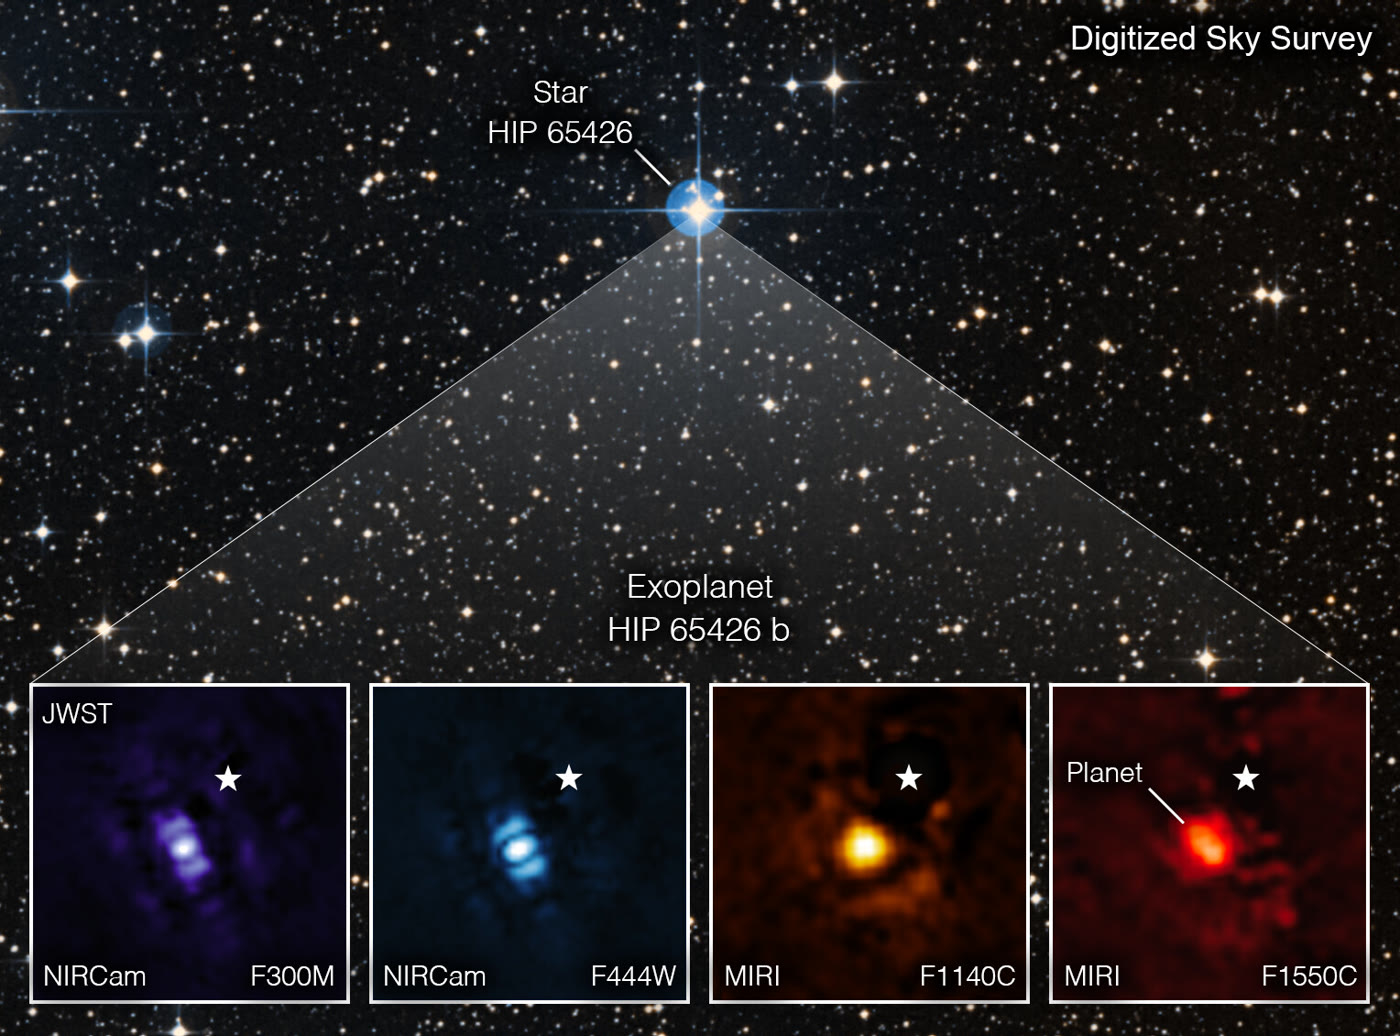
\includegraphics[width=0.86\linewidth]{images/book5/b3-hip65426b.jpg}
\par\smallskip{\small El primer exoplaneta fotografiado por el telescopio espacial James Webb,
HIP~65426~b, en cuatro filtros infrarrojos (abajo; arriba, el campo de la estrella en un
sondeo del cielo desde tierra); la luz de la estrella, en la posición del símbolo de
estrella, queda bloqueada por los
\omterm{def:b3:exoplanets:imaging}{coronógrafos}. El planeta es un gigante gaseoso joven de unas 6 a 8
masas de Júpiter, de entre 15 y 20 millones de años, a unas cien veces más lejos de su estrella
de lo que la Tierra está del Sol. Imagen NASA/ESA/CSA,
A~Carter (UCSC), equipo de ERS~1386 y A.~Pagan (STScI), CC
BY~4.0.}\label{fig:b3:exoplanets:hip65426}
\end{omfigure}
% ledger: photo:b3-hip65426b

Un cuarto método usa la gravedad como lente. Cuando una estrella pasa casi exactamente
delante de otra más lejana, su gravedad curva la luz de la
estrella de fondo y la hace brillar durante unas semanas; un planeta de la estrella que actúa de lente
añade un breve destello.

\begin{definition}[Microlente gravitatoria; radio de Einstein]\label{def:b3:exoplanets:microlensing}
La \emph{microlente gravitatoria}\index{microlente gravitatoria} es el
aumento temporal del brillo de una estrella de fondo cuando una estrella de primer plano, la
lente, pasa cerca de la línea de visión; las imágenes que forma están demasiado
juntas para resolverse. El \emph{radio de Einstein}\index{radio de Einstein}
es el radio angular $\theta_\mathrm E$ del anillo en el que una lente puntual
de masa $M$ situada a la distancia $D_L$ desviaría una fuente situada a la
distancia $D_S$ exactamente detrás de ella:
\[
\theta_\mathrm E = \sqrt{\frac{4GM}{c^2}\,\frac{D_S - D_L}{D_L D_S}} .
\]
\end{definition}

\begin{proposition}[Amplificación de una lente puntual]\label{prop:b3:exoplanets:magnification}
Una fuente situada a la distancia angular $u\,\theta_\mathrm E$ de una lente puntual
se aclara en el factor
\[
A(u) = \frac{u^2 + 2}{u\sqrt{u^2 + 4}} .
\]
\end{proposition}

\admitted

Ambos resultados provienen de la desviación de la luz por una masa en
la relatividad general. Para una lente de media masa solar, situada a mitad de camino
de una fuente que dista \qty{8}{kpc}, $\theta_\mathrm E = \qty{0.71}{mas}$, y el anillo de Einstein,
a la distancia de la lente, tiene un radio de \qty{2.9}{au}. Para
$u = 1$ la fuente se aclara 1.34 veces, y para $u = 0.1$, diez veces. Un
planeta situado cerca del anillo de Einstein de su estrella añade una desviación breve
a la curva de luz. Así, la microlente permite encontrar planetas a unas pocas unidades
astronómicas de sus estrellas, planetas fríos que los tránsitos y las velocidades radiales no detectan,
pero cada evento ocurre una sola vez y nunca se repite. En un evento de 2003,
publicado al año siguiente, una desviación que duró unos siete días solo se explicó
mediante un compañero de $\num{0.0039}$ veces la masa de la lente: un planeta de unas
1.5 masas de Júpiter situado a unas \qty{3}{au}
de su estrella.
% ledger: const:G, const:c, sun:mass, iau:parsec, const:au, bond04:ogle235

\begin{omfigure}
\centering
\begin{tikzpicture}[scale=0.95]
\fill (0,0) circle (0.06) node[below=2pt, font=\scriptsize] {fuente};
\fill[omDef] (3.2,0) circle (0.09); \node[font=\scriptsize, omDef] at (3.2,-1.15) {lente};
\draw[omDef] (3.2,0) ellipse (0.12 and 0.9);
\fill (6.4,0) circle (0.06) node[below=2pt, font=\scriptsize] {observador};
\draw[thick, orange!80!black] (0,0) -- (3.2,0.9) -- (6.4,0);
\draw[thick, orange!80!black] (0,0) -- (3.2,-0.9) -- (6.4,0);
\draw[densely dashed, black!50] (6.4,0) -- (0,1.8) node[left, font=\scriptsize] {imagen};
\draw[densely dotted, black!50] (0,0) -- (6.4,0);
\draw[<->] (3.55,0) -- (3.55,0.9) node[midway, right, font=\scriptsize] {$R_\mathrm E$};
\draw[<->, black!60] (0,-1.5) -- (3.2,-1.5) node[midway, below, font=\scriptsize] {$D_S - D_L$};
\draw[<->, black!60] (3.2,-1.5) -- (6.4,-1.5) node[midway, below, font=\scriptsize] {$D_L$};
\end{tikzpicture}\hfill
\begin{tikzpicture}
\begin{axis}[width=0.48\linewidth, height=0.42\linewidth,
  xmin=-3, xmax=3, ymin=0.8, ymax=12, ymode=log,
  ytick={1,2,5,10}, yticklabels={1,2,5,10},
  xlabel={tiempo ($t_\mathrm E$)}, ylabel={amplificación $A$},
  tick label style={font=\scriptsize}, label style={font=\small},
  legend style={font=\scriptsize, at={(0.5,-0.30)}, anchor=north, legend columns=3, draw=none, cells={anchor=west}, /tikz/every even column/.append style={column sep=1em}}]
\addplot[thick, omDef] table[x=t_tE, y=A01] {figdata/out/bachelor-3-rv_transit-lens.dat};
\addlegendentry{$u_0 = 0.1$}
\addplot[thick, dashed, red!70!black] table[x=t_tE, y=A03] {figdata/out/bachelor-3-rv_transit-lens.dat};
\addlegendentry{$0.3$}
\addplot[thick, dotted, black] table[x=t_tE, y=A10] {figdata/out/bachelor-3-rv_transit-lens.dat};
\addlegendentry{$1$}
\end{axis}
\end{tikzpicture}
\par\smallskip{\small Izquierda: la geometría de una lente gravitatoria, no a escala; los rayos
procedentes de la fuente pasan junto a la lente a aproximadamente el \omterm{def:b3:exoplanets:microlensing}{radio de Einstein}
$R_\mathrm E = \theta_\mathrm E D_L$ y llegan al observador, que ve la fuente desplazada hacia la imagen.
Derecha: la amplificación de una fuente puntual por una lente puntual frente al tiempo,
en unidades del tiempo $t_\mathrm E$ que tarda la lente en desplazarse un \omterm{def:b3:exoplanets:microlensing}{radio de Einstein},
para tres distancias de máximo acercamiento
$u_0$ (en \omterm{def:b3:exoplanets:microlensing}{radios de Einstein}).}\label{fig:b3:exoplanets:microlensing}
\end{omfigure}

Cada método tiene su propio sesgo, y el catálogo de planetas conocidos los refleja.
Las velocidades radiales favorecen los planetas masivos cercanos a sus estrellas;
los tránsitos favorecen los planetas grandes cercanos a sus estrellas, y necesitan que la órbita esté de canto;
la microlente encuentra planetas a unas pocas unidades astronómicas;
la imagen encuentra gigantes jóvenes a decenas o cientos de unidades astronómicas.
La figura siguiente muestra el resultado: cada método ocupa su propia región, y los planetas del Sistema Solar
caen en su mayoría en los huecos que quedan entre ellas.

\begin{dated}{2026}
El 23 de octubre de 2026 el NASA Exoplanet Archive
recogía 6451 planetas confirmados. Por método de descubrimiento: 4785 por tránsitos, 1204 por
velocidad radial, 292 por microlente, 98 por imagen, 29 por \omterm{def:b3:exoplanets:ttv}{variaciones del tiempo de tránsito}
y el resto por métodos más raros, entre ellos los primeros de todos, hallados en 1992 alrededor
de un púlsar mediante la medida del tiempo de sus pulsos. Los primeros descubrimientos
por velocidad radial datan de 1995, por tránsito de 2002,
y por microlente e imagen de 2004.
\end{dated}
% ledger: data:b5-pscomp

\begin{omfigure}
\centering
\begin{tikzpicture}
\begin{axis}[width=0.86\linewidth, height=0.56\linewidth,
  xmode=log, ymode=log, xmin=0.004, xmax=2000, ymin=0.02, ymax=1e5,
  legend image post style={scale=2.2},
  xlabel={semieje mayor (au)}, ylabel={masa o masa mínima ($M_\oplus$)},
  tick label style={font=\scriptsize}, label style={font=\small},
  legend style={font=\scriptsize, at={(0.5,-0.20)}, anchor=north, legend columns=4, draw=none, cells={anchor=west}, /tikz/every even column/.append style={column sep=1em}}]
\addplot[only marks, mark=*, mark size=0.6pt, omDef, opacity=0.6] table[x=a_au, y=mass] {figdata/out/bachelor-3-exoplanet_archive-ma-tr.dat};
\addlegendentry{tránsito}
\addplot[only marks, mark=*, mark size=0.6pt, red!70!black, opacity=0.6] table[x=a_au, y=mass] {figdata/out/bachelor-3-exoplanet_archive-ma-rv.dat};
\addlegendentry{velocidad radial}
\addplot[only marks, mark=triangle*, mark size=1.2pt, green!45!black] table[x=a_au, y=mass] {figdata/out/bachelor-3-exoplanet_archive-ma-ml.dat};
\addlegendentry{microlente}
\addplot[only marks, mark=diamond*, mark size=1.5pt, orange!85!black] table[x=a_au, y=mass] {figdata/out/bachelor-3-exoplanet_archive-ma-im.dat};
\addlegendentry{imagen}
\addplot[only marks, mark=square*, mark size=1.6pt, black, forget plot] table[x=a_au, y=mass] {figdata/out/bachelor-3-exoplanet_archive-solar.dat};
\node[font=\scriptsize, anchor=west, fill=white, inner sep=1pt] at (axis cs:1.15,1.0) {Tierra};
\node[font=\scriptsize, anchor=east, fill=white, inner sep=1pt] at (axis cs:0.63,0.82) {Venus};
\node[font=\scriptsize, anchor=east, fill=white, inner sep=1pt] at (axis cs:0.34,0.055) {Mercurio};
\node[font=\scriptsize, anchor=west, fill=white, inner sep=1pt] at (axis cs:1.75,0.107) {Marte};
\node[font=\scriptsize, anchor=west, fill=white, inner sep=1pt] at (axis cs:6.0,318) {Júpiter};
\node[font=\scriptsize, anchor=west, fill=white, inner sep=1pt] at (axis cs:11,95) {Saturno};
\node[font=\scriptsize, anchor=north, fill=white, inner sep=1pt] at (axis cs:25,11) {Urano, Neptuno};
\end{axis}
\end{tikzpicture}
\par\smallskip{\small Planetas confirmados con masa medida (o \omterm{def:b3:exoplanets:rv}{masa mínima}) y semieje mayor,
por método de descubrimiento (NASA Exoplanet Archive, 23 de octubre de 2026:
1691 por tránsito, 1151 por velocidad radial, 286 por microlente, 94 por imagen),
con los planetas del Sistema Solar (cuadrados negros). Se omiten las masas predichas
a partir de una \omterm{def:b3:exoplanets:mass-radius}{relación masa--radio}.
Esta investigación ha utilizado el NASA Exoplanet Archive,
que es operado por el Instituto de Tecnología de California, bajo contrato con la
Administración Nacional de Aeronáutica y del Espacio dentro del
Programa de Exploración de Exoplanetas.}\label{fig:b3:exoplanets:methods}
\end{omfigure}
% ledger: data:b5-pscomp, planet:Mercury.mass, planet:Venus.mass, planet:Earth.mass, planet:Mars.mass, planet:Jupiter.mass, planet:Saturn.mass, planet:Uranus.mass, planet:Neptune.mass, planet:Mercury.dist, planet:Venus.dist, planet:Earth.dist, planet:Mars.dist, planet:Jupiter.dist, planet:Saturn.dist, planet:Uranus.dist, planet:Neptune.dist

\section{Lo que se ha encontrado}\label{sec:b3:exoplanets:found}

La primera sorpresa fue la de los \omterm{def:b3:exoplanets:classes}{júpiteres calientes}, planetas gigantes en órbitas de
unos pocos días. 51~Pegasi~b no puede haberse formado tan cerca de su estrella; debe de
haberse formado más lejos, quizá a unas pocas unidades astronómicas, más allá de la
línea de nieve de su disco, y migró hacia el interior por su interacción con
el disco, tal como había predicho la teoría.
% ledger: nobel19:migration

\begin{definition}[Júpiter caliente; supertierra; subneptuno]\label{def:b3:exoplanets:classes}
Un \emph{júpiter caliente}\index{júpiter caliente} es un planeta gigante en una órbita cercana,
que suele considerarse con una \omterm{def:b3:exoplanets:rv}{masa mínima} superior a 0.1 masas de Júpiter y un periodo
menor que diez días. Una \emph{supertierra}\index{supertierra} es un planeta
mayor que la Tierra pero menor que el \omterm{def:b3:exoplanets:radius-valley}{valle de radios}, es decir, de hasta
unos 1.5 a 2 radios terrestres, y por ello probablemente rocoso. Un \emph{subneptuno}\index{subneptuno}
es un planeta por encima del \omterm{def:b3:exoplanets:radius-valley}{valle de radios} pero menor que Neptuno, de unos 2 a
4 radios terrestres, cuyo radio exige una envoltura de gases ligeros o
volátiles.
\end{definition}
% ledger: wright12:hj, fulton17:gap, planet:Neptune.diameter, planet:Earth.diameter

\begin{definition}[Tasa de ocurrencia]\label{def:b3:exoplanets:occurrence}
La \emph{tasa de ocurrencia}\index{tasa de ocurrencia} de una clase de planetas es
el número medio de tales planetas por estrella, o la fracción de estrellas que
albergan uno, en un intervalo dado de tamaño (o masa) y periodo, una vez
corregidos los recuentos de un sondeo por los planetas que no pudo detectar:
los que tienen órbitas no alineadas para un tránsito, y los demasiado pequeños o
demasiado lejanos para verse.
\end{definition}

Los \omterm{def:b3:exoplanets:classes}{júpiteres calientes}, prominentes en el catálogo porque son los más fáciles de
encontrar, son raros: un sondeo por el \omterm{def:b3:exoplanets:rv}{método de la velocidad radial} de estrellas cercanas
de tipo solar las halló en \qty[separate-uncertainty=true]{1.2 \pm 0.38}{\percent} de las estrellas. Los planetas pequeños son
comunes. Al buscar en las curvas de luz de \num{42000} estrellas observadas por el
telescopio espacial Kepler, un estudio halló 603 planetas, diez de ellos del tamaño de la Tierra (de 1 a 2
radios terrestres) y que recibían entre una y cuatro veces la insolación de la
Tierra; una vez corregido por la probabilidad de tránsito y por los planetas que la
búsqueda no detectaría, \qty[separate-uncertainty=true]{11 \pm 4}{\percent} de las estrellas de tipo solar albergan un
planeta de ese tipo.
% ledger: wright12:hj, petigura13:eta

Los tamaños de los planetas pequeños no se reparten de manera uniforme. Entre los planetas de órbita cercana
medidos con precisión, los de 1.5 a 2.0 radios terrestres son al menos dos veces
más escasos que los inmediatamente menores o mayores.

\begin{definition}[Valle de radios]\label{def:b3:exoplanets:radius-valley}
El \emph{valle de radios}\index{valle de radios} es el déficit de planetas
con radios de entre unos 1.5 y 2.0 radios terrestres entre los planetas con
periodos menores de unos cien días; separa las \omterm{def:b3:exoplanets:classes}{supertierras}
de los \omterm{def:b3:exoplanets:classes}{subneptunos}.
\end{definition}
% ledger: fulton17:gap

El valle se interpreta como la huella del escape. Un núcleo rocoso que nace con una
envoltura de hidrógeno y helio de apenas unos pocos por ciento de su masa tiene el doble
radio del núcleo desnudo. Cerca de una estrella joven y activa, tal envoltura
se calienta y se pierde por \omterm{def:b3:planetary-atmospheres:hydrodynamic}{escape hidrodinámico}: por la
radiación de alta energía de la estrella durante los primeros cien millones de años
(fotoevaporación), o por el calor del propio núcleo en enfriamiento (pérdida de masa
impulsada por el núcleo). Los modelos agrupan los planetas en núcleos desnudos de unos 1.3
radios terrestres y planetas del doble de ese tamaño; quedan pocos en medio.
Los dos mecanismos dependen de forma distinta de la estrella, y los planetas en torno a estrellas de
tipos distintos podrían distinguirlos.
% ledger: owen17:valley, ginzburg18:core-powered

\begin{omfigure}
\centering
\begin{tikzpicture}
\begin{axis}[name=pr, width=0.50\linewidth, height=0.50\linewidth,
  xmode=log, ymode=log, xmin=1, xmax=100, ymin=0.8, ymax=4,
  ytick={1,1.5,2,3,4}, yticklabels={1,1.5,2,3,4},
  xlabel={periodo (días)}, ylabel={radio ($R_\oplus$)},
  tick label style={font=\scriptsize}, label style={font=\small},
  title={(a)}, title style={font=\small}]
\fill[black!10] (axis cs:1,1.5) rectangle (axis cs:100,2.0);
\addplot[only marks, mark=*, mark size=0.5pt, omDef, opacity=0.7] table[x=period, y=radius] {figdata/out/bachelor-3-exoplanet_archive-pr.dat};
\end{axis}
\begin{axis}[at={(pr.east)}, anchor=west, xshift=0.09\linewidth,
  width=0.42\linewidth, height=0.50\linewidth,
  xmode=log, xmin=0.8, xmax=4, ymin=0, ymax=185,
  xtick={1,1.5,2,3,4}, xticklabels={1,1.5,2,3,4},
  xlabel={radio ($R_\oplus$)}, ylabel={número de planetas},
  tick label style={font=\scriptsize}, label style={font=\small},
  title={(b)}, title style={font=\small}]
\fill[black!10] (axis cs:1.5,0) rectangle (axis cs:2.0,185);
\addplot[const plot mark left, thick, omDef, fill=omDef!25] table[x=r, y=n] {figdata/out/bachelor-3-exoplanet_archive-histstep.dat} \closedcycle;
\end{axis}
\end{tikzpicture}
\par\smallskip{\small (a)~Planetas en tránsito con radios conocidos con una precisión mejor que
\qty{10}{\percent}, en torno a estrellas menores de dos radios solares, con
periodos de 1 a 100 días (2370 planetas, NASA Exoplanet Archive, 23
de octubre de 2026); en sombreado, el \omterm{def:b3:exoplanets:radius-valley}{valle de radios} de 1.5 a 2.0 radios terrestres.
(b)~Los mismos planetas contados en 20 intervalos de igual anchura en $\log R$.
Los recuentos no están corregidos por los planetas que los sondeos no detectan, que son
más numerosos entre los pequeños; el valle se aprecia de todos modos.}\label{fig:b3:exoplanets:valley}
\end{omfigure}
% ledger: data:b5-pscomp, fulton17:gap

\begin{definition}[Relación masa--radio]\label{def:b3:exoplanets:mass-radius}
La \emph{relación masa--radio}\index{relación masa--radio} de una
composición es el radio de un planeta de esa composición en función de
su masa, calculado a partir de las ecuaciones de estado de sus materiales en
equilibrio hidrostático; un planeta medido se compara con las
relaciones de las composiciones candidatas.
\end{definition}

Un planeta rocoso se comprime por su propio peso, y su radio crece
más lentamente que $M^{1/3}$. Un ajuste a modelos de planetas de dos capas construidos sobre
el modelo sísmico de la Tierra da $R/R_\oplus = (1.07 - 0.21\,C)
(M/M_\oplus)^{1/3.7}$, para masas de 1 a 8 masas terrestres y una fracción de masa del núcleo
$C$ de 0 a 0.4; ajustado a la Tierra, a Venus y a unos pocos
exoplanetas, da $C = 0.26 \pm 0.07$. Un
planeta de hierro es más pequeño a la misma masa; un planeta compuesto a mitad por agua, mayor;
una envoltura de hidrógeno de apenas el dos por ciento de la masa convierte un planeta de
cinco masas terrestres y \num{2.6} radios terrestres, del tamaño de un
\omterm{def:b3:exoplanets:classes}{subneptuno}. La degeneración es real: un radio y una masa dan una
densidad, y varias mezclas de hierro, roca, agua y gas pueden compartirla.
El planeta rocoso Kepler-10~b, de 3.24 masas terrestres y 1.47 radios terrestres,
tiene una densidad media de \qty{5.6}{g.cm^{-3}}; el gigante gaseoso WASP-39~b,
de 89 masas terrestres y 14.3 radios terrestres, \qty{0.17}{g.cm^{-3}}.
% ledger: zeng16:rocky, data:b5-zeng, data:b5-pscomp

\begin{omfigure}
\centering
\begin{tikzpicture}
\begin{axis}[width=0.86\linewidth, height=0.58\linewidth,
  xmode=log, ymode=log, xmin=0.3, xmax=5000, ymin=0.5, ymax=25,
  ytick={0.5,1,2,4,10,20}, yticklabels={0.5,1,2,4,10,20},
  xlabel={masa ($M_\oplus$)}, ylabel={radio ($R_\oplus$)},
  tick label style={font=\scriptsize}, label style={font=\small},
  legend style={font=\scriptsize, at={(0.5,-0.20)}, anchor=north, legend columns=3, draw=none, cells={anchor=west}, /tikz/every even column/.append style={column sep=1em}}]
\addplot[only marks, mark=*, mark size=0.6pt, black!35, forget plot] table[x=mass, y=radius] {figdata/out/bachelor-3-exoplanet_archive-mr.dat};
\addplot[thick, black] table[x=mass, y=radius] {figdata/out/bachelor-3-exoplanet_archive-zeng-iron.dat};
\addlegendentry{hierro puro}
\addplot[thick, brown!70!black] table[x=mass, y=radius] {figdata/out/bachelor-3-exoplanet_archive-zeng-earthlike.dat};
\addlegendentry{roca semejante a la terrestre}
\addplot[thick, omDef] table[x=mass, y=radius] {figdata/out/bachelor-3-exoplanet_archive-zeng-water50.dat};
\addlegendentry{50\,\% de agua}
\addplot[thick, dashed, orange!85!black] table[x=mass, y=radius] {figdata/out/bachelor-3-exoplanet_archive-zeng-h2-2pc.dat};
\addlegendentry{roca + 2\,\% de hidrógeno}
\addplot[only marks, mark=square*, mark size=1.8pt, red!70!black] table[x=mass, y=radius] {figdata/out/bachelor-3-exoplanet_archive-solar.dat};
\addlegendentry{Sistema Solar}
\node[font=\scriptsize, anchor=north west] at (axis cs:1.05,0.97) {Tierra};
\node[font=\scriptsize, anchor=south east] at (axis cs:0.80,0.97) {Venus};
\node[font=\scriptsize, anchor=south east, fill=white, inner sep=1pt] at (axis cs:13.5,4.3) {Urano, Neptuno};
\node[font=\scriptsize, anchor=east, fill=white, inner sep=1pt] at (axis cs:80,9.45) {Saturno};
\node[font=\scriptsize, anchor=north, fill=white, inner sep=1pt] at (axis cs:318,10.3) {Júpiter};
\end{axis}
\end{tikzpicture}
\par\smallskip{\small Masa y radio de 1078 planetas en tránsito cuya
masa se mide con una precisión mejor que \qty{25}{\percent} y el radio
con una precisión mejor que \qty{10}{\percent} (en gris; NASA Exoplanet Archive, 23 de octubre de 2026),
con las curvas de modelo de L.~Zeng y otros (2016, 2019): hierro puro;
roca semejante a la terrestre, con un tercio de hierro y dos tercios de silicato; mitad de agua sobre
un núcleo de ese tipo, a \qty{500}{K}; un núcleo semejante al terrestre con una envoltura de hidrógeno de
\qty{2}{\percent} de su masa, a \qty{500}{K}. Cuadrados rojos: los planetas del
Sistema Solar (Mercurio y Marte quedan fuera de la escala, a la
izquierda).}\label{fig:b3:exoplanets:mass-radius}
\end{omfigure}
% ledger: data:b5-pscomp, data:b5-zeng, planet:Earth.mass, planet:Earth.diameter, planet:Venus.mass, planet:Venus.diameter, planet:Jupiter.mass, planet:Jupiter.diameter, planet:Saturn.mass, planet:Saturn.diameter, planet:Uranus.mass, planet:Uranus.diameter, planet:Neptune.mass, planet:Neptune.diameter

\section{Atmósferas}\label{sec:b3:exoplanets:atmospheres}

Un planeta en tránsito puede pesarse y medirse; también puede olerse.
Durante un tránsito, un anillo delgado de la atmósfera del planeta se interpone
frente a la estrella, y la luz estelar la atraviesa filtrada. A las longitudes de onda
en las que un gas de la atmósfera absorbe, el anillo es opaco a mayor altura,
y el planeta parece más grande.

\begin{definition}[Espectroscopía de transmisión; eclipse secundario]\label{def:b3:exoplanets:transmission}
La \emph{espectroscopía de transmisión}\index{espectroscopía de transmisión} mide
la \omterm{def:b3:exoplanets:transit}{profundidad del tránsito} en función de la longitud de onda, para detectar los gases de la
atmósfera que atraviesa la luz estelar en el limbo del planeta. Un
\emph{eclipse secundario}\index{eclipse secundario} es el paso de un
planeta por detrás de su estrella, media órbita después del tránsito en una
órbita circular; la caída del flujo del sistema mide entonces la luz del
lado diurno del planeta.
\end{definition}

\begin{proposition}[Señal de transmisión]\label{prop:b3:exoplanets:transmission}
Una atmósfera de altura de escala $H \ll R_p$, opaca a lo largo de $n$ alturas de escala
más en la longitud de onda de una banda de absorción que en las longitudes de onda vecinas,
profundiza allí el tránsito en
\[
\Delta\delta \approx n\,\frac{2HR_p}{R_\star^2} .
\]
\end{proposition}

\begin{proof}
El radio aparente del planeta crece de $R_p$ a $R_p + nH$, así que la
profundidad $(R_p + nH)^2/R_\star^2$ crece en $(2nHR_p + n^2H^2)/R_\star^2$,
que es $2nHR_p/R_\star^2$ cuando $nH \ll R_p$.
\end{proof}

La altura de escala $H = kT/\bar m g$ es grande en un planeta caliente de gravedad
baja y aire ligero de hidrógeno, y pequeña en un planeta frío y denso de aire
pesado. Para la Tierra vista frente al Sol, con $H = \qty{8}{km}$,
cada altura de escala añade 0.2 partes por millón; para un gigante gaseoso caliente e hinchado,
varios cientos.
% ledger: planet:Earth.diameter, sun:R

\begin{proposition}[Profundidad del eclipse secundario]\label{prop:b3:exoplanets:eclipse}
Si el lado diurno de un planeta radía como un cuerpo negro a la temperatura
$T_d$ y la estrella como uno a $T_\star$, el \omterm{def:b3:exoplanets:transmission}{eclipse secundario} a la
longitud de onda $\lambda$ tiene la profundidad
\[
\delta_\mathrm{ecl} \approx \left(\frac{R_p}{R_\star}\right)^2
  \frac{B_\lambda(T_d)}{B_\lambda(T_\star)},
\]
con $B_\lambda$ la ley de Planck, despreciando la luz reflejada por el planeta.
\end{proposition}

\begin{proof}
Justo antes del eclipse, el observador recibe la luz de la estrella, en
proporción a $\pi R_\star^2 B_\lambda(T_\star)$, más la del lado diurno,
en proporción a $\pi R_p^2 B_\lambda(T_d)$; durante el eclipse, solo la
de la estrella. La caída fraccionaria es el cociente del término del planeta
entre el de la estrella, siendo pequeño el del planeta.
\end{proof}

El eclipse es más profundo en el infrarrojo, donde el planeta frío resulta
más brillante en relación con su estrella: da la temperatura del lado diurno, y
un lado diurno caliente junto a un lado nocturno frío revela una atmósfera delgada o ausente
que no reparte el calor.

\begin{dated}{2023}
En 2022 el espectro de transmisión del gigante gaseoso WASP-39~b, medido
entre 3.0 y \qty{5.5}{\micro m} por el telescopio espacial James Webb,
mostró una banda de absorción prominente del dióxido de carbono a
\qty{4.3}{\micro m}, a 26 desviaciones típicas, donde las fotometrías anteriores
solo habían insinuado el gas: su primera identificación clara en
la atmósfera de un exoplaneta. En 2023 se observaron cinco \omterm{def:b3:exoplanets:transmission}{eclipses secundarios}
de TRAPPIST-1~b, de tamaño terrestre, que recibe cuatro veces la luz solar de
la Tierra desde una estrella fría y pequeña; se midieron a \qty{15}{\micro m}. Encajan con
el calor reirradiado solo desde el lado diurno, sin dióxido de carbono
detectable: el planeta tiene poca o ninguna atmósfera que lleve calor a su
lado nocturno.
\end{dated}
% ledger: jwst23:wasp39-co2, greene23:trappist1b

Los planetas rocosos de las zonas habitables de las estrellas pequeñas
están al alcance de estos métodos, en el límite. Si conservaron su
atmósfera frente a los procesos de escape del capítulo anterior es ahora una
cuestión observacional.

\section{Ejercicios}

\begin{exercise}[$\star$]\label{exo:b3:exoplanets:1}
(a)~Calcúlese la semiamplitud de la velocidad radial del Sol causada por
Júpiter (masa \qty{1898e24}{kg}, periodo \num{4331}~días, excentricidad
0.049) y por la Tierra (masa \qty{5.97e24}{kg}, periodo \num{365.2}~días,
excentricidad 0.017). La masa del Sol es \qty{1.9884e30}{kg}.
(b)~Conviértanse las precisiones \qty{3.5}{km/h} y \qty{0.35}{km/h} a
metros por segundo, y compárense.
\end{exercise}

\begin{exercise}[$\star$]\label{exo:b3:exoplanets:2}
(a)~Calcúlese la profundidad de tránsito de Júpiter (radio \qty{71492}{km}) y de
la Tierra (radio \qty{6378}{km}) sobre el Sol (radio
\qty{695700}{km}). (b)~Calcúlese la probabilidad de que un observador colocado al
azar vea cada uno de ellos en tránsito, con radios orbitales de \num{778.5}
y \qty{149.6}{\mega km}.
\end{exercise}

\begin{exercise}[$\star$]\label{exo:b3:exoplanets:3}
51~Pegasi~b produce en su estrella una semiamplitud de la velocidad radial de
\qty{59}{m.s^{-1}}, con un periodo de \qty{4.23}{d}. Tomando la masa de la
estrella igual a la del Sol, calcúlense la \omterm{def:b3:exoplanets:rv}{masa mínima} del planeta, en masas de
Júpiter y en masas terrestres, y el radio de su órbita.
\end{exercise}

\begin{exercise}[$\star$]\label{exo:b3:exoplanets:4}
Una estrella de media masa solar a \qty{4}{kpc} actúa como lente sobre una
estrella a \qty{8}{kpc} ($\qty{1}{pc} = \qty{3.0857e16}{m}$). (a)~Calcúlese su
\omterm{def:b3:exoplanets:microlensing}{radio de Einstein} en milisegundos de arco y el radio del anillo de Einstein,
en unidades astronómicas, a la distancia de la lente. (b)~Calcúlese la
amplificación para $u = 1$, $0.5$ y $0.1$. (c)~¿Cuánto tarda la lente en
atravesar un \omterm{def:b3:exoplanets:microlensing}{radio de Einstein} si se desplaza a través de la línea de visión a
\qty{200}{km.s^{-1}}?
\end{exercise}

\begin{exercise}[$\star\star$]\label{exo:b3:exoplanets:5}
Un planeta de razón de radios $p = 0.12$ orbita una estrella de una masa solar y
un radio solar en \qty{3.0}{d}. (a)~Calcúlese $a/R_\star$. (b)~Calcúlense
$T_{14}$ y $T_{23}$ para $b = 0$ y para $b = 0.7$, y la inclinación en el
segundo caso. (c)~¿Cómo permite la forma de la curva de luz distinguir un
tránsito central de uno rasante?
\end{exercise}

\begin{exercise}[$\star\star$]\label{exo:b3:exoplanets:6}
A partir de las masas y los radios del Exoplanet Archive, calcúlense las
densidades medias de TRAPPIST-1~b (1.374 masas terrestres, 1.116 radios
terrestres), Kepler-10~b (3.24, 1.47), WASP-39~b (89.31, 14.34) y HD~209458~b (232.0,
15.58), con $M_\oplus = \qty{5.97e24}{kg}$ y $R_\oplus =
\qty{6378}{km}$. ¿Cuáles son rocosos y cuáles gaseosos?
\end{exercise}

\begin{exercise}[$\star\star$]\label{exo:b3:exoplanets:7}
La velocidad radial de una estrella con un planeta en una órbita excéntrica
varía entre $+\qty{50.4}{m.s^{-1}}$ y $-\qty{9.6}{m.s^{-1}}$, y la velocidad del
centro de masas del sistema es \qty{12.4}{m.s^{-1}}. Utilizando la forma
excéntrica del teorema, calcúlese $K$ y $e\cos\omega$. ¿Por qué la media de los
dos extremos puede diferir de $\gamma$?
\end{exercise}

\begin{exercise}[$\star\star$]\label{exo:b3:exoplanets:8}
WASP-39~b tiene 89.31 masas terrestres y 14.34 radios terrestres; su estrella de
0.939 radios solares. Tómese una temperatura de \qty{1100}{K} y una
masa molecular media de \qty{2.3}{u} para su atmósfera. (a)~Calcúlense su gravedad,
su altura de escala y su profundidad de tránsito. (b)~Calcúlese la señal de
transmisión de una altura de escala, y la de una banda de absorción de dos
alturas de escala, en partes por millón.
\end{exercise}

\begin{exercise}[$\star\star$]\label{exo:b3:exoplanets:9}
TRAPPIST-1~b tiene un radio de 1.116 radios terrestres; su estrella, de 0.1192
radios solares y \qty{2566}{K}. Calcúlese la profundidad de su \omterm{def:b3:exoplanets:transmission}{eclipse secundario} a
\qty{15}{\micro m} para un lado diurno a \qty{400}{K} y a \qty{500}{K}
($hc/k = \qty{0.014388}{m.K}$). ¿Por qué una medida de la profundidad
es un termómetro?
\end{exercise}

\begin{exercise}[$\star\star\star$]\label{exo:b3:exoplanets:10}
Una enana roja imaginaria tiene 0.2 masas solares, 0.2 radios solares y una
luminosidad de \num{0.005} luminosidades solares. (a)~¿A qué distancia recibe un
planeta el flujo estelar de la Tierra, y cuál es su periodo?
(b)~Calcúlese la semiamplitud causada allí por un planeta de una masa terrestre,
y compárese con el efecto de la Tierra sobre el Sol. (c)~Calcúlese la
profundidad de tránsito de un planeta del tamaño de la Tierra. ¿Por qué estas
estrellas son objetivos preferentes en la búsqueda de planetas rocosos en zonas habitables?
\end{exercise}

\begin{exercise}[$\star\star\star$]\label{exo:b3:exoplanets:11}
Para la ley de \omterm{def:b3:exoplanets:limb}{oscurecimiento del limbo} cuadrática, demuéstrese que la intensidad
media del disco es $I(1)(1 - u_1/3 - u_2/6)$. Dedúzcase la profundidad, en unidades
de $p^2$, de un planeta pequeño en $r = 0$, $0.5$ y $0.9$ para $u_1 = 0.40$,
$u_2 = 0.25$. ¿Qué error cometería un modelo de disco uniforme en el radio de un
planeta observado en mitad del tránsito con $b = 0$?
\end{exercise}

\begin{exercise}[$\star\star\star$]\label{exo:b3:exoplanets:12}
Un sondeo observó \num{42000} estrellas similares al Sol y las buscó en busca de
planetas del tamaño de la Tierra que recibieran entre una y cuatro veces la luz
solar terrestre, es decir, en órbitas de 0.5 a \qty{1}{au}. (a)~Calcúlese la
probabilidad de tránsito a 0.5, 0.7 y \qty{1}{au}. (b)~Si el \qty{11}{\percent} de las
estrellas alberga uno de tales planetas, a unas \qty{0.7}{au}, ¿cuántos transitan?
(c)~El sondeo encontró diez. ¿Qué mide la diferencia y por qué debe corregirse la
\omterm{def:b3:exoplanets:occurrence}{tasa de ocurrencia} por ella?
\end{exercise}

\section{Problema: un planeta alrededor de la lámpara de Selene}

\begin{problem}[{Problema de fin de semana --- pesar, medir y olfatear un
planeta inventado}]
\label{pb:b3:exoplanets:1}
La lámpara de Selene es una enana~K inventada de masa 0.80 masas solares, radio
0.76 radios solares y temperatura efectiva \qty{5000}{K}. Un
sondeo de velocidad radial detecta que su velocidad varía sinusoidalmente con
un período de \qty{12.0}{d} y una semiamplitud de \qty{2.59}{m.s^{-1}}. Un
telescopio espacial observa después tránsitos del mismo período, de profundidad
\num{838} partes por millón y duración total $T_{14} = \qty{3.23}{h}$.
Tómense $M_\odot = \qty{1.9884e30}{kg}$, $R_\odot = \qty{695700}{km}$,
$L_\odot = \qty{3.828e26}{W}$, $M_\oplus = \qty{5.97e24}{kg}$,
$R_\oplus = \qty{6378}{km}$.

\medskip\noindent\textbf{Parte I --- La velocidad radial.}
\begin{enumerate}
\item Calcúlese el radio de la órbita, en metros y en
  unidades astronómicas, despreciando la masa del planeta frente a la de la estrella.
\item Calcúlese la velocidad orbital del planeta.
\item Calcúlese la \omterm{def:b3:exoplanets:rv}{masa mínima} del planeta, en masas terrestres.
\item Calcúlese el radio de la órbita de la estrella alrededor del centro de
  masas, y compruébese que reproduce la semiamplitud observada.
\item ¿Cuántas veces supera la señal una precisión de
  \qty{1}{m.s^{-1}} y de \qty{0.1}{m.s^{-1}}?
\item Si la órbita tuviera $e = 0.2$ con el mismo $K$, ¿en cuánto variaría la
  \omterm{def:b3:exoplanets:rv}{masa mínima}?
\end{enumerate}

\medskip\noindent\textbf{Parte II --- El tránsito.}
\begin{enumerate}[resume]
\item Calcúlese la razón de radios $p = R_p/R_\star$.
\item Calcúlese el radio del planeta, en kilómetros y en radios terrestres.
\item Calcúlese $a/R_\star$.
\item Calcúlese la duración de un tránsito central ($b = 0$).
\item A partir del $T_{14}$ observado, calcúlese el \omterm{def:b3:exoplanets:transit}{parámetro de impacto}.
\item Calcúlese la inclinación de la órbita.
\item ¿Cuál era la probabilidad de que este planeta transitara, vista desde una
  dirección aleatoria?
\end{enumerate}

\medskip\noindent\textbf{Parte III --- ¿De qué está hecho?}
\begin{enumerate}[resume]
\item Calcúlese la masa real del planeta.
\item Calcúlese su densidad media.
\item En la curva del modelo rocoso de tipo terrestre, un planeta de esta masa tendría
  un radio de 1.74 radios terrestres. Compárese y dígase qué debe
  contener el planeta además de roca.
\item ¿Dónde se sitúa el planeta respecto al \omterm{def:b3:exoplanets:radius-valley}{valle de radios}? ¿Es
  una \omterm{def:b3:exoplanets:classes}{supertierra} o un \omterm{def:b3:exoplanets:classes}{subneptuno}?
\item Calcúlese su gravedad superficial.
\end{enumerate}

\medskip\noindent\textbf{Parte IV --- Su atmósfera.}
\begin{enumerate}[resume]
\item Calcúlese la luminosidad de la estrella, en vatios y en luminosidades
  solares.
\item Calcúlese el flujo estelar que recibe el planeta, relativo al de la
  Tierra. ¿Está en la zona habitable?
\item Con un albedo de Bond de 0.3, calcúlese su temperatura de equilibrio.
\item Calcúlese la altura de escala de una atmósfera de hidrógeno y helio
  (masa molecular media \qty{2.3}{u}) a esa temperatura.
\item Calcúlese la señal de transmisión de una altura de escala, y de una
  banda de agua situada a dos alturas de escala, en partes por millón.
\item Calcúlese lo mismo para una atmósfera de vapor de agua (\qty{18}{u}). ¿Cuál de
  los dos podría distinguir de un espectro plano un telescopio espacial con una precisión de unas diez partes por
  millón?
\item Dese la densidad media del planeta, en gramos por centímetro cúbico, con
  dos cifras significativas.
\end{enumerate}
\end{problem}
% ledger: sun:mass, sun:R, sun:L, planet:Earth.mass, planet:Earth.diameter, const:G, const:kB, const:sigma, nist:u, data:b5-zeng, fulton17:gap, eso:espresso
